
\documentclass[border=10pt, 12pt]{standalone}
\usepackage[svgnames]{xcolor}
\usepackage{amsmath}
\usepackage{pgfplots}
\pgfplotsset{compat=newest}
\usepackage[sfdefault]{FiraSans}
\usepackage{FiraMono}
\renewcommand*\familydefault{\sfdefault}
\begin{document}
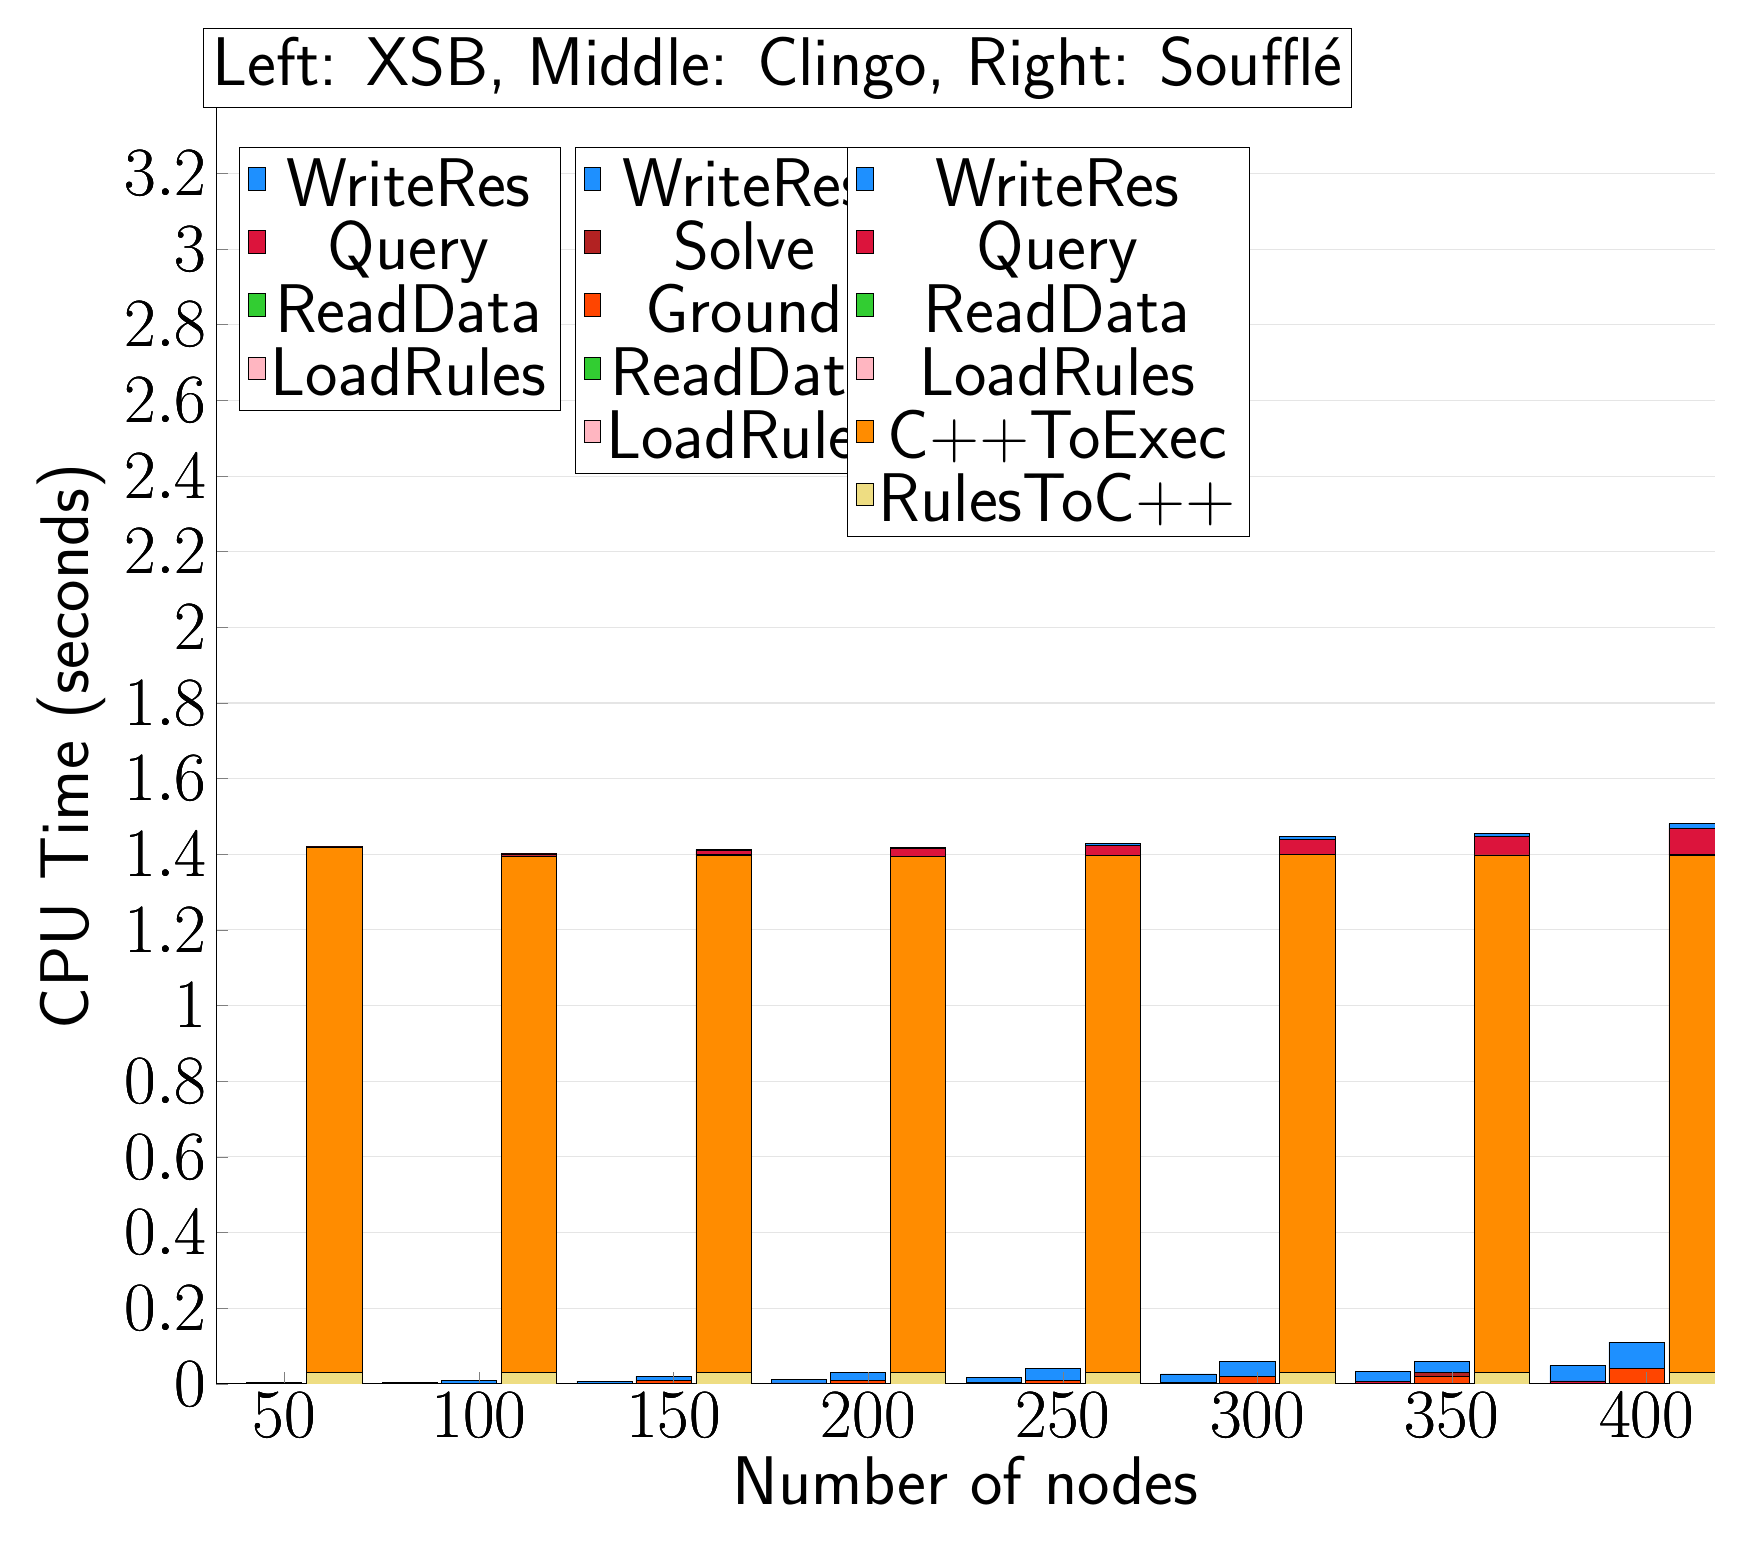
\begin{tikzpicture}
	\begin{axis}[bar shift=-25pt,
			ybar stacked,
			width=1.7\textwidth,
			bar width=0.7cm,
			ymajorgrids, tick align=inside,
			major grid style={draw=gray!20},
			xtick=data,
			ymin=0, ymax=3.3720000000000003,
			axis x line*=bottom,
			axis y line*=left,
			enlarge x limits=0.05,
			legend style={
					at={(0.23, 0.97)},
					anchor=north east,
					legend columns=1,
					font=\Huge,
				},
			ylabel={CPU Time (seconds)},
			xlabel={Number of nodes},
			label style={font=\Huge},
			tick label style={font=\Huge},
		]
		\addlegendimage{fill=DodgerBlue, draw=black, line width=0.2pt}
		\addlegendentry{WriteRes}
		\addlegendimage{fill=Crimson, draw=black, line width=0.2pt}
		\addlegendentry{Query}
		\addlegendimage{fill=LimeGreen, draw=black, line width=0.2pt}
		\addlegendentry{ReadData}
		\addlegendimage{fill=LightPink, draw=black, line width=0.2pt}
		\addlegendentry{LoadRules}
		\addplot +[fill=LightPink, draw=black, line width=0.2pt] coordinates {
				(50, 0.0006118999999999996)
				(100, 0.0006121999999999999)
				(150, 0.0006184)
				(200, 0.0006035000000000004)
				(250, 0.0006374000000000004)
				(300, 0.0006142)
				(350, 0.0006053000000000001)
				(400, 0.0006104999999999998)
			};
		\addplot +[fill=LimeGreen, draw=black, line width=0.2pt] coordinates {
				(50, 0.00021480000000000018)
				(100, 0.0002908000000000001)
				(150, 0.0003622)
				(200, 0.0004423000000000002)
				(250, 0.000511599999999999)
				(300, 0.0005992)
				(350, 0.0006670999999999997)
				(400, 0.0007891000000000006)
			};
		\addplot +[fill=Crimson, draw=black, line width=0.2pt] coordinates {
				(50, 0.0001294999999999996)
				(100, 0.0004586999999999998)
				(150, 0.0009027999999999998)
				(200, 0.0016041)
				(250, 0.0022034000000000003)
				(300, 0.0033685)
				(350, 0.0042209)
				(400, 0.0064233)
			};
		\addplot +[fill=DodgerBlue, draw=black, line width=0.2pt] coordinates {
				(50, 0.0007276000000000007)
				(100, 0.0027120000000000004)
				(150, 0.0055442)
				(200, 0.010098300000000001)
				(250, 0.013196100000000002)
				(300, 0.021485499999999998)
				(350, 0.026588800000000003)
				(400, 0.040131299999999995)
			};
	\end{axis}

	\begin{axis}[bar shift=-3.7pt,
			ybar stacked,
			width=1.7\textwidth,
			bar width=0.7cm,
			ymajorgrids, tick align=inside,
			major grid style={draw=none},
			xtick=data,
			ymin=0, ymax=3.3720000000000003,
			axis x line*=none,
			axis y line*=none,
			enlarge x limits=0.05,
			legend style={
					at={(0.454, 0.97)},
					anchor=north east,
					legend columns=1,
					font=\Huge,
				},
			label style={font=\Huge},
			tick label style={font=\Huge},
		]
		\addlegendimage{fill=DodgerBlue, draw=black, line width=0.2pt}
		\addlegendentry{WriteRes}
		\addlegendimage{fill=FireBrick, draw=black, line width=0.2pt}
		\addlegendentry{Solve}
		\addlegendimage{fill=OrangeRed, draw=black, line width=0.2pt}
		\addlegendentry{Ground}
		\addlegendimage{fill=LimeGreen, draw=black, line width=0.2pt}
		\addlegendentry{ReadData}
		\addlegendimage{fill=LightPink, draw=black, line width=0.2pt}
		\addlegendentry{LoadRules}
		\addplot +[fill=LightPink, draw=black, line width=0.2pt] coordinates {
				(50, 0.0)
				(100, 0.0)
				(150, 0.0)
				(200, 0.0)
				(250, 0.0)
				(300, 0.0)
				(350, 0.0)
				(400, 0.0)
			};
		\addplot +[fill=LimeGreen, draw=black, line width=0.2pt] coordinates {
				(50, 0.0)
				(100, 0.0)
				(150, 0.0009999999999999998)
				(200, 0.0)
				(250, 0.0)
				(300, 0.0)
				(350, 0.0)
				(400, 0.0)
			};
		\addplot +[fill=OrangeRed, draw=black, line width=0.2pt] coordinates {
				(50, 0.0009999999999999998)
				(100, 0.0)
				(150, 0.008999999999999998)
				(200, 0.009999999999999997)
				(250, 0.009999999999999997)
				(300, 0.019999999999999997)
				(350, 0.019999999999999997)
				(400, 0.03999999999999999)
			};
		\addplot +[fill=FireBrick, draw=black, line width=0.2pt] coordinates {
				(50, 0.0)
				(100, 0.0)
				(150, 0.0)
				(200, 0.0)
				(250, 0.0)
				(300, 0.0)
				(350, 0.010000000000000004)
				(400, 0.0)
			};
		\addplot +[fill=DodgerBlue, draw=black, line width=0.2pt] coordinates {
				(50, 0.0029999999999999996)
				(100, 0.009999999999999997)
				(150, 0.010000000000000004)
				(200, 0.020000000000000007)
				(250, 0.030000000000000006)
				(300, 0.039999999999999994)
				(350, 0.029999999999999992)
				(400, 0.07000000000000002)
			};
	\end{axis}

	\begin{axis}[bar shift=18pt,
			ybar stacked,
			width=1.7\textwidth,
			bar width=0.7cm,
			ymajorgrids, tick align=inside,
			major grid style={draw=none},
			xtick=data,
			ymin=0, ymax=3.3720000000000003,
			axis x line*=none,
			axis y line*=none,
			enlarge x limits=0.05,
			legend style={
					at={(0.69, 0.97)},
					anchor=north east,
					legend columns=1,
					font=\Huge,
				},
			label style={font=\Huge},
			tick label style={font=\Huge},
		]
		\addlegendimage{fill=DodgerBlue, draw=black, line width=0.2pt}
		\addlegendentry{WriteRes}
		\addlegendimage{fill=Crimson, draw=black, line width=0.2pt}
		\addlegendentry{Query}
		\addlegendimage{fill=LimeGreen, draw=black, line width=0.2pt}
		\addlegendentry{ReadData}
		\addlegendimage{fill=LightPink, draw=black, line width=0.2pt}
		\addlegendentry{LoadRules}
		\addlegendimage{fill=DarkOrange, draw=black, line width=0.2pt}
		\addlegendentry{C++ToExec}
		\addlegendimage{fill=LightGoldenrod, draw=black, line width=0.2pt}
		\addlegendentry{RulesToC++}
		\addplot +[fill=LightGoldenrod, draw=black, line width=0.2pt] coordinates {
				(50, 0.031000000000000007)
				(100, 0.030000000000000006)
				(150, 0.030000000000000006)
				(200, 0.030000000000000006)
				(250, 0.030000000000000006)
				(300, 0.030000000000000006)
				(350, 0.030000000000000006)
				(400, 0.030000000000000006)
			};
		\addplot +[fill=DarkOrange, draw=black, line width=0.2pt] coordinates {
				(50, 1.3870000000000005)
				(100, 1.3649999999999998)
				(150, 1.3680000000000003)
				(200, 1.364)
				(250, 1.367)
				(300, 1.3690000000000002)
				(350, 1.3670000000000002)
				(400, 1.3670000000000004)
			};
		\addplot +[fill=LightPink, draw=black, line width=0.2pt] coordinates {
				(50, 1.11e-05)
				(100, 0.0)
				(150, 0.0)
				(200, 0.0)
				(250, 0.0)
				(300, 0.0)
				(350, 0.0)
				(400, 0.0)
			};
		\addplot +[fill=LimeGreen, draw=black, line width=0.2pt] coordinates {
				(50, 0.00042899999999999997)
				(100, 0.000603)
				(150, 0.0007983)
				(200, 0.0009653999999999999)
				(250, 0.0011419)
				(300, 0.0013221)
				(350, 0.0014648)
				(400, 0.0017973)
			};
		\addplot +[fill=Crimson, draw=black, line width=0.2pt] coordinates {
				(50, 0.0012752)
				(100, 0.005269500000000001)
				(150, 0.0114678)
				(200, 0.0200389)
				(250, 0.026190700000000004)
				(300, 0.039286600000000005)
				(350, 0.04879399999999999)
				(400, 0.06986789999999998)
			};
		\addplot +[fill=DodgerBlue, draw=black, line width=0.2pt] coordinates {
				(50, 0.00048130000000000004)
				(100, 0.0014197999999999997)
				(150, 0.0027275)
				(200, 0.0042571)
				(250, 0.0051936000000000005)
				(300, 0.007281900000000001)
				(350, 0.008761)
				(400, 0.012331400000000001)
			};
	\end{axis}


	\node[anchor=south, draw, fill=white] at (rel axis cs:0.42,1) {\Huge Left: XSB, Middle: Clingo, Right: Soufflé};
\end{tikzpicture}
\end{document}
